%%% "Activity-Dependent Plasticity in Morphogenetically-Grown Recurrent Networks"
%%% Medvid S.O., Valenia A.I., Glybovets M.M.
%%%
%%% arXiv version
%%% Compile with: pdflatex main_arxiv && pdflatex main_arxiv

\pdfoutput=1
\documentclass[sigconf,nonacm]{acmart}

% Remove ACM-specific metadata for workshop submission
\settopmatter{printacmref=false}
\renewcommand\footnotetextcopyrightpermission[1]{}
\pagestyle{plain}

\usepackage{booktabs}
\usepackage{multirow}
\usepackage{graphicx}
\usepackage{xcolor}
\usepackage{amsmath}

\begin{document}

\title{Activity-Dependent Plasticity in Morphogenetically-Grown Recurrent Networks}

\author{Sergii Medvid}
\affiliation{%
  \institution{National University of Kyiv-Mohyla Academy}
  \city{Kyiv}
  \country{Ukraine}
}
\email{s.medvid@ukma.edu.ua}

\author{Andrii Valenia}
\affiliation{%
  \institution{National University of Kyiv-Mohyla Academy}
  \city{Kyiv}
  \country{Ukraine}
}
\email{a.valenia@ukma.edu.ua}

\author{Mykola Glybovets}
\affiliation{%
  \institution{National University of Kyiv-Mohyla Academy}
  \city{Kyiv}
  \country{Ukraine}
}
\email{glib@ukma.edu.ua}

\begin{CCSXML}
<ccs2012>
<concept>
<concept_id>10010147.10010257.10010293.10010294</concept_id>
<concept_desc>Computing methodologies~Neural networks</concept_desc>
<concept_significance>500</concept_significance>
</concept>
<concept>
<concept_id>10010147.10010257.10010293.10010319</concept_id>
<concept_desc>Computing methodologies~Bio-inspired approaches</concept_desc>
<concept_significance>300</concept_significance>
</concept>
</ccs2012>
\end{CCSXML}

\ccsdesc[500]{Computing methodologies~Neural networks}
\ccsdesc[300]{Computing methodologies~Bio-inspired approaches}

\begin{abstract}
Developmental approaches to neural architecture search grow functional networks from compact genomes through self-organisation, but the resulting networks operate with fixed post-growth weights.
We characterise Hebbian and anti-Hebbian plasticity across 50{,}000 morphogenetically grown recurrent controllers (5M+ configurations on CartPole and Acrobot), then test whether co-evolutionary experiments---where plasticity parameters are encoded in the geno\-me and evolved alongside the developmental architecture---recover these patterns independently.
Our characterisation reveals that (1)~anti-Hebbian plasticity significantly outperforms Hebbian for competent networks (Cohen's $d = 0.53$--$0.64$), (2)~regret (fraction of oracle improvement lost under the best fixed setting) reaches 52--100\%, and (3)~plasticity's role shifts from fine-tuning to genuine adaptation under non-stationarity.
Co-evolution independently discovers these patterns: on CartPole, 70\% of runs evolve anti-Hebbian plasticity ($p = 0.043$); on Acrobot, evolution finds near-zero $\eta$ with mixed signs---exactly matching the characterisation.
A random-RNN control shows that anti-Hebbian dominance is generic to small recurrent networks, but the \emph{degree} of topology-dependence is developmental-specific: regret is 2--6$\times$ higher for morphogenetically grown networks than for random graphs with matched topology statistics.
\end{abstract}

\keywords{developmental neural networks, synaptic plasticity, morphogenetic self-organisation, neuroevolution, indirect encoding}

\maketitle

%% ============================================================
\section{Introduction}
\label{sec:intro}

Developmental approaches to neural architecture search---including Neural Developmental Programs (NDP)~\cite{najarro2023ndp}, HyperNCA~\cite{najarro2022hypernca}, and MorphoNAS~\cite{glybovets2026morphonas}---encode compact genomes that unfold into functional neural networks through developmental processes. These systems demonstrate that self-organising developmental rules can produce effective controllers from far fewer parameters than direct weight specification, echoing the genomic bottleneck observed in biological brains~\cite{zador2019critique}.

In MorphoNAS, as in NDP and HyperNCA, the network topology and weights are fixed once development completes. This contrasts with biological neural circuits, where activity-dependent synaptic plasticity enables within-lifetime adaptation~\cite{hebb1949organization}. Recent work on Hebbian neuroevolution~\cite{najarro2020meta} has shown that evolving plasticity rules can produce adaptive agents, but this work operates on fixed-topology networks rather than developmentally grown architectures. Palm et~al.~\cite{palm2021testing} tested the genomic bottleneck hypothesis with Hebbian meta-learning but found that naive bottleneck application to plasticity rules leads to poor performance, suggesting a difficult joint optimisation problem.

Two fundamental questions arise. First, \textbf{can post-development\-al plasticity meaningfully improve morphogenetically grown networks, and if so, under what conditions?} Second, \textbf{can evolutionary optimisation discover the right plasticity parameters for each architecture, and does this interaction differ between developmental and random networks?} These questions are central to evolving self-organising systems: structural self-organisation (development) and functional self-organisation (plasticity) may interact in ways that neither uniform parameter tuning nor isolated analysis can reveal.

We present a systematic characterisation of synaptic plasticity in developmental networks at population scale, followed by co-evolutionary experiments that test whether evolutionary optimisation recovers the characterisation patterns. We use MorphoNAS~\cite{glybovets2026morphonas} as our experimental platform. Its reaction-diffusion dynamics~\cite{turing1952chemical} produce structurally diverse topologies from compact genomes, making it a suitable testbed for the broader class of developmental encodings. We evaluate Hebbian and anti-Hebbian plasticity across 50{,}000 morphogenetically grown CartPole controllers under three task conditions (static, 10$\times$ pole mass, 2$\times$ gravity), replicate key findings on 5{,}000 Acrobot controllers, then test whether co-evolving plasticity parameters alongside the developmental genome recovers the characterisation patterns. A random-RNN control disentangles developmental from generic network effects. Our contributions are:

\begin{itemize}
  \item A stratified characterisation across 3.75M evaluations revealing anti-Hebbian dominance (Cohen's $d = 0.53$--$0.64$), topology-dependent regret (52--100\%), and a functional role-shift from fine-tuning to genuine within-lifetime adaptation under non-stationarity.
  \item Co-evolutionary validation: when plasticity parameters are encoded in the genome and evolved, evolution independently discovers anti-Hebbian dominance on CartPole ($p = 0.043$) and the correct $\eta$ scale on both benchmarks.
  \item A random-RNN control showing that anti-Hebbian dominance is generic to small RNNs, but the \emph{degree} of topology-dependence (regret) is 2--6$\times$ higher for developmental networks, confirming that morphogenetic structure creates uniquely diverse plasticity interactions.
\end{itemize}

%% ============================================================
\section{Related Work}
\label{sec:related}

\textbf{Developmental neural networks.}
Indirect encodings that grow neural networks through developmental processes have a rich history in evolutionary computation. Stanley's NEAT~\cite{stanley2002evolving} complexifies topology through mutation, while HyperNEAT~\cite{stanley2009hypercube} uses compositional pattern-producing networks to exploit geometric regularities. Neural Cellular Automata (NCA)~\cite{mordvintsev2020growing} demonstrated that self-organising update rules can grow complex patterns from local interactions; Neural Developmental Programs (NDP)~\cite{najarro2023ndp} and HyperNCA~\cite{najarro2022hypernca} extend this to grow functional neural networks through self-assembling developmental processes. MorphoNAS~\cite{glybovets2026morphonas} takes a complementary developmental path, using Turing-type reaction-diffusion morphogen dynamics~\cite{turing1952chemical} rather than learned update rules. Nisioti et~al.~\cite{nisioti2024growing} showed that maintaining neuronal diversity during NDP growth---via intrinsic hidden states and lateral inhibition---is essential for producing functional controllers, providing independent evidence that the developmental process shapes the structural heterogeneity of the resulting networks. In all these systems, weights are typically fixed during task execution.

\textbf{Plasticity in neuroevolution.}
Soltoggio et~al.~\cite{soltoggio2018born} survey the field of evolved plastic networks, identifying Hebbian and neuromodulated plasticity as the dominant paradigms. Najarro and Risi~\cite{najarro2020meta} demonstrated that Hebbian learning rules evolved via meta-learning can produce agents that adapt within their lifetime---but on fixed-topology random networks, not developmentally grown ones. Plantec et~al.~\cite{plantec2024evolving} introduced the Lifelong Neural Developmental Program (LNDP), combining graph-transformer-based development with experience-dependent structural plasticity, enabling networks to add and prune connections during task execution. Garc{\'\i}a~N{\'u}{\~n}ez et~al.~\cite{garcianunez2025time} proposed time-modulated Hebbian learning (tm-HL) for classic control tasks, introducing a decay term $\mu_t = e^{-\lambda t}$ that transitions networks from high plasticity to fixed weights over the agent's lifetime; they used $\lambda = 0.01$---the same value we find effective for weight decay. However, their work uses fixed feedforward architectures and does not test anti-Hebbian rules. Our work complements theirs by characterising plasticity across 50{,}000 \emph{developmentally grown} topologies, revealing that the interaction between plasticity and network structure---rather than plasticity parameters alone---is the dominant factor.

\textbf{The genomic bottleneck.}
Zador~\cite{zador2019critique} argued that biological brains leverage compact genomic encodings that specify wiring rules rather than individual weights, with experience fine-tuning pre-wired circuits. Palm et~al.~\cite{palm2021testing} tested whether a genomic bottleneck improves Hebbian meta-learning but found the joint optimisation problem difficult under their approach. Our work takes a different approach: we first characterise how simple plasticity interacts with the topology already compressed through morphogenetic development, then test whether encoding plasticity parameters in the genome and co-evolving them alongside the developmental architecture can exploit this interaction.

%% ============================================================
\section{Experimental Design}
\label{sec:design}

\subsection{MorphoNAS Developmental System}

We use MorphoNAS~\cite{glybovets2026morphonas}, a morphogenetic neural architecture search system where a compact genome (54 parameters for 3 morphogens) encodes morphogen secretion rates, diffusion tensors, cross-inhibi\-tion coefficients, cell-fate thresholds, and axon growth rules. Starting from a single progenitor cell on a 2D toroidal grid, each developmental iteration involves morphogen secretion, spatial diffusion, competitive cross-inhibition (producing reaction-diffusion dynamics and symmetry breaking), local cell-fate decisions (division, differentiation, or quiescence), and chemotactic axon growth with distance-dependent weight initialisation ($w = \max(0.01,\; c/(1+d))$). After a genome-specified number of iterations, the process yields a recurrent neural network (RNN) whose topology and weights emerge entirely from local chemical interactions (Figure~\ref{fig:morphonas}). The process is fully deterministic: the same genome always produces the same network. Crucially, the 54 parameters do not specify individual neurons or connections---they encode morphogen dynamics whose self-organising interactions constrain the phenotype space to morphogenetically plausible topologies. Different genomes produce structurally distinct networks, and it is these structural differences that make the interaction with plasticity topology-dependent (Section~\ref{sec:results}). See~\cite{glybovets2026morphonas} for full details.

\begin{figure}[t]
  \centering
  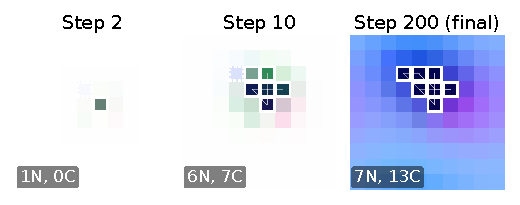
\includegraphics[width=\columnwidth]{figures/morphonas_development.pdf}
  \caption{Developmental dynamics of a MorphoNAS network on a $10 \times 10$ grid. Background colour encodes morphogen concentrations (RGB = 3 morphogens); white squares = neurons; white lines = connections. From a single progenitor cell (Step~2), reaction-diffusion dynamics drive cell division, differentiation, and chemotactic axon growth, producing a 7-neuron, 13-connection recurrent controller by Step~200.}
  \label{fig:morphonas}
\end{figure}

\subsection{Task and Network Pool}

The resulting networks are evaluated as controllers on CartPole-v1 (OpenAI Gymnasium~\cite{towers2024gymnasium}), where the objective is to balance a pole on a cart for up to 500~timesteps. CartPole is deliberately chosen as a minimal substrate: its simplicity isolates the development-plasticity interaction from task complexity, while mid-episode physics perturbations (Section~\ref{sec:adaptation}) reveal how plasticity's role changes with environmental demands.

We generated 50{,}000 networks from \emph{randomly sampled} genomes (no evolutionary selection; each genome drawn independently from the MorphoNAS parameter space). We stratified networks by baseline CartPole performance (mean reward over 20~episodes without plasticity):

\begin{itemize}
  \item \textbf{Weak} ($r < 200$): $N = 47{,}638$ (95.3\%)
  \item \textbf{Low-mid} ($200 \le r < 350$): $N = 1{,}235$
  \item \textbf{High-mid} ($350 \le r < 450$): $N = 256$
  \item \textbf{Near-perfect} ($450 \le r < 475$): $N = 102$
  \item \textbf{Perfect} ($r \ge 475$): $N = 769$
\end{itemize}

That 95.3\% of random genomes produce Weak networks indicates that, in our setting, \emph{viable topology is the primary determinant of performance}: while 15\% of Weak networks show marginal improvement, the developmental process must produce a functional architecture before plasticity can contribute substantially.

\subsection{Plasticity Protocol}

We apply a Hebbian plasticity rule after development completes. At each propagation timestep during task execution, weights are updated according to:
\begin{equation}
  \Delta w_{ij} = \eta \cdot x_i \cdot x_j - \lambda \cdot w_{ij}
  \label{eq:hebb}
\end{equation}
where $\eta$ is the learning rate (positive for Hebbian, negative for anti-Hebbian), $x_i, x_j$ are pre- and post-synaptic activations, and $\lambda$ is a weight decay coefficient that acts as a stability mechanism.

Each network is evaluated under a rigorous protocol: (1)~baseline measurement with plasticity disabled, (2)~plasticity-enabled evaluation over 20~episodes with fixed seeds (42--61), (3)~fitness comparison. The improvement $\Delta r$ is the difference in mean reward between the plasticity-enabled and baseline evaluations. All experiments ran on AWS c6i.4xlarge instances (16~vCPU, Intel Xeon 8375C); the full experimental programme (characterisation, co-evolution, and random-RNN control) required approximately 7{,}700 core-hours.

\subsection{Parameter Sweeps}

We conducted three CartPole experimental phases at increasing resolution, followed by an Acrobot replication.

\textbf{Primary sweep} (CartPole): 50{,}000 networks $\times$ 75 parameter combinations ($\eta \in [-0.05, +0.05]$, 15 non-uniform levels; $\lambda \in \{0, 10^{-5}, 10^{-4}, 10^{-3}, 10^{-2}\}$) = 3{,}750{,}000 evaluations.

\textbf{Extended validation} (CartPole): 2{,}862 non-Weak networks (including borderline cases near stratum boundaries) $\times$ 248-point grid ($\eta \in [-0.5, +0.5]$, 31 levels; $\lambda \in \{0, \ldots, 0.1\}$, 8 levels) = 709{,}776 evaluations. Used for cross-validated regret estimation.

\textbf{Non-stationarity sweep} (CartPole): 2{,}362 non-Weak networks $\times$ 22-point grid (anti-Hebbian range only), evaluated on two variants where physics change abruptly at timestep~200 with no signal to the network: (a)~pole mass increases 10$\times$ (0.1$\to$1.0\,kg), affecting inertial dynamics, and (b)~gravity doubles (9.8$\to$20.0\,m/s$^2$), uniformly scaling forces. Together: 103{,}928 evaluations.

\textbf{Adaptation control} (CartPole): To isolate genuine adaptation from robustness, we evaluated the same 2{,}362 networks with plasticity \emph{disabled} during Phase~1 (pre-switch) and enabled only at the switch point (OFF$\to$ON protocol), on both non-stationary variants. A dose-response experiment varied the switch time (100, 200, 300, 400) under heavy-pole to test whether more post-switch adaptation time yields larger benefits. Together: 155{,}892 evaluations.

\textbf{Acrobot replication}: To test cross-task generalisation, we repeated the analysis on Acrobot-v1 (6-dimensional observations, 3 discrete actions) using a $20 \times 20$ developmental grid. We sampled 5{,}000 random genomes; 513 non-Weak networks were evaluated on a coarse 22-point grid followed by an extended 248-point micro-$\eta$ grid ($|\eta| \in [5 \times 10^{-5}, 0.1]$; $\lambda \in [0, 0.1]$), under both static and non-stationary conditions (2$\times$ lower-link mass at step~50).

Across all characterisation experiments, the total evaluation budget exceeds 5 million plasticity configurations.

\subsection{Co-Evolutionary Validation}
\label{sec:coevolution_design}

To test whether evolutionary optimisation independently recovers the characterisation findings, we ran a genetic algorithm evolving MorphoNAS genomes under three conditions (30 independent runs each, population~50, 200~generations):
\begin{itemize}
  \item \textbf{Condition~A} (no plasticity): standard MorphoNAS GA, fitness evaluated with frozen weights.
  \item \textbf{Condition~B} (fixed plasticity): same GA, but fitness evaluated with fixed anti-Hebbian plasticity ($\eta = -0.01$, $\lambda = 0.01$ for CartPole; $\eta = -0.001$, $\lambda = 0.05$ for Acrobot---the recommended defaults from the characterisation).
  \item \textbf{Condition~C} (co-evolved plasticity): the genome is extended with two plasticity parameters ($\eta$, $\lambda$) that are mutated and crossed over alongside the developmental genome. On CartPole: $\eta \in [-0.5, +0.5]$, $\lambda \in [0, 0.1]$; on Acrobot: $\eta \in [-0.1, +0.1]$, $\lambda \in [0, 0.1]$.
\end{itemize}
CartPole experiments used a $10 \times 10$ grid (matching the characterisation), and Acrobot used $20 \times 20$. Selection: top-20\%; elitism: 2; mutation rate: 0.3.
Total: 180 GA runs (90 per benchmark), each 10{,}050 fitness evaluations.

\subsection{Random-RNN Control}
\label{sec:random_rnn_design}

To disentangle developmental from generic network effects, we generated 11{,}810 random directed graphs matched to the topology statistics (neuron count, connection count) of 2{,}362 competent MorphoNAS CartPole networks (5~random RNNs per source network). Weights were drawn from $\text{Uniform}[0.01, 1.0]$, matching MorphoNAS's $w = \max(0.01, c/(1{+}d))$ range but without distance-dependent structure. We applied the same 75-point plasticity grid as the primary characterisation sweep to all competent random RNNs.

%% ============================================================
\section{Characterisation Results}
\label{sec:results}

\subsection{Stratified Plasticity Impact}
\label{sec:stratified}

Table~\ref{tab:stratified} presents the per-stratum impact of plasticity under \emph{oracle} tuning---exhaustive per-network grid search for the best $(\eta, \lambda)$ pair, representing an upper bound on achievable benefit.

\begin{table}[t]
\caption{CartPole plasticity impact by performance stratum under per-network oracle parameters. Regret: fraction of oracle improvement lost when using the single best fixed parameter pair instead.}
\label{tab:stratified}
\small
\begin{tabular}{@{}lrrrrr@{}}
\toprule
Stratum & $N$ & Oracle $\Delta r$ & \% Impr. & Best $\eta$ & Regret \\
\midrule
Weak       & 47{,}638 & $+2.2$   & 15\% & $+0.05$ & 59\%  \\
Low-mid    & 1{,}235  & $+35.7$  & 50\% & $-0.05$ & 52\%  \\
\textbf{High-mid} & \textbf{256} & $\mathbf{+60.6}$ & \textbf{93\%} & $\mathbf{-0.05}$ & \textbf{86\%} \\
Near-perf. & 102      & $+22.5$  & 84\% & $-0.005$ & 89\% \\
Perfect    & 769      & $+7.7$   & 20\% & ---     & 100\% \\
\bottomrule
\end{tabular}
\end{table}

Three key patterns emerge. First, plasticity \emph{cannot rescue weak topologies}: networks with non-functional architectures show negligible improvement regardless of plasticity parameters. In our experiments, topology produced by morphogenetic development is the primary determinant of viability. Second, \emph{competent networks benefit substantially}: up to 93\% of High-mid networks improve under oracle tuning, with mean gains of +60.6 reward points. Third, \emph{per-network parameter heterogeneity is large}: regret under fixed parameters ranges from 52\% (Low-mid) to 100\% (Perfect), indicating that no single parameter setting captures the oracle potential.

Table~\ref{tab:stratified} reports conservative estimates from the 75-point primary sweep; the best $\eta$ for Low-mid and High-mid falls at the grid boundary ($|\eta| = 0.05$). The extended 248-point validation grid, which widens the range to $|\eta| \le 0.5$, yields higher oracle improvements: $+73.4$ for Low-mid and $+86.3$ for High-mid. Split-half cross-validation (oracle selected on odd-numbered episodes, evaluated on even) confirmed that 74--92\% of the oracle advantage reflects genuine per-network heterogeneity, not overfitting to noise. Under ceiling-corrected normalisation (gain as fraction of available headroom), High-mid networks capture 87\% of their improvement room and Near-perfect 78\%, indicating that oracle plasticity nearly saturates the performance gap.

The magnitude of oracle gains enables \emph{stratum transitions}: under per-network tuning, a majority of High-mid and Near-perfect networks reach the Perfect stratum ($r \ge 475$), suggesting that plasticity can close the gap between ``competent but imperfect'' and ``fully functional'' controllers---a qualitative shift in behaviour, not merely a marginal improvement.

However, plasticity carries asymmetric risk. Harm rates increase with baseline competence: 1.3\% (Weak), 18.5\% (Low-mid), 42.0\% (High-mid), 48.5\% (Near-perfect). The worst-case configurations ($\eta > 0$, $\lambda = 0$) produce severe degradation, with mean normalised harm of $-0.17$ to $-0.24$ ($-85$ to $-120$ raw reward points) for competent strata. This asymmetry---where the networks most likely to benefit are also most vulnerable to harm---further motivates per-network parameter selection over fixed configurations.

\subsection{Anti-Hebbian Dominance}

\begin{figure}[t]
  \centering
  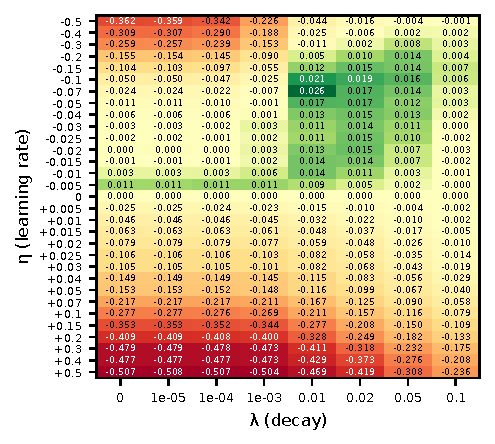
\includegraphics[width=\columnwidth]{figures/heatmap_high_mid.pdf}
  \caption{CartPole High-mid stratum: mean $\Delta r$ across the $\eta \times \lambda$ grid (248-point extended grid). Anti-Hebbian ($\eta < 0$) with moderate decay ($\lambda = 0.01$) yields the best results. Hebbian ($\eta > 0$) is consistently harmful.}
  \label{fig:heatmap}
\end{figure}

\begin{figure}[t]
  \centering
  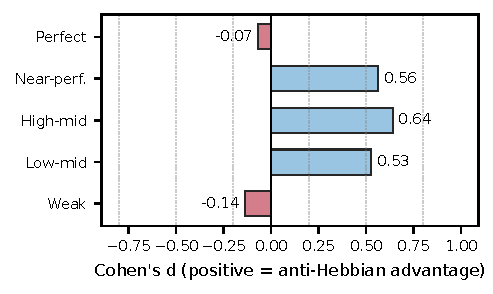
\includegraphics[width=\columnwidth]{figures/cohens_d.pdf}
  \caption{CartPole: Cohen's $d$ (anti-Hebbian $-$ Hebbian) by stratum. Anti-Hebbian significantly outperforms Hebbian for competent strata ($d = 0.53$--$0.64$, all $p < 0.001$). The effect reverses for Weak and Perfect networks with small magnitudes.}
  \label{fig:cohens_d}
\end{figure}

Anti-Hebbian plasticity ($\eta < 0$) significantly outperforms Hebbian ($\eta > 0$) for all competent strata (Figure~\ref{fig:cohens_d}). On the extended 248-point grid, the effect is substantial: Cohen's $d = 0.53$ for Low-mid, $d = 0.64$ for High-mid, and $d = 0.56$ for Near-perfect (all $p < 0.001$). The effect reverses for Weak ($d = -0.14$) and Perfect ($d = -0.07$) networks, though with small absolute magnitudes.

Kruskal-Wallis variance decomposition on the extended parameter grid~\cite{derrac2011practical} reveals that learning rate ($\eta$) explains 22--35\% of variance in competent strata ($\varepsilon^2 = H/(N{-}1)$), while decay ($\lambda$) explains less than 5\%. This indicates that \emph{the sign and magnitude of $\eta$ is the critical design choice}, while decay acts primarily as a safety mechanism. The sweet spot of $\lambda = 0.01$ reduces harm rates by 3--8$\times$ compared to $\lambda = 0$ with minimal reduction in peak benefit.

What drives the anti-Hebbian advantage? We tested two mechanistic hypotheses. First, that anti-Hebbian plasticity acts as a decorrelation mechanism; we found no relationship between initial weight magnitude and anti-Hebbian preference ($p = 0.56$, Mann-Whitney). Second, that Hebbian updates overshoot by reinforcing existing correlations too aggressively; correlational evidence is consistent: networks whose optimal $\eta$ is positive (Hebbian) exhibit 2.6$\times$ larger per-step weight changes than anti-Hebbian-preferring networks ($p < 10^{-25}$; per-stratum $d = 0.34$--$0.87$). The lowest weight-change quintile shows 93\% anti-Hebbian preference versus 64\% in the highest quintile. While not dispositive, this pattern is consistent with \emph{magnitude moderation}---anti-Hebbian updates counteract co-activation rather than amplifying it, preventing the runaway weight growth that makes Hebbian updates harmful for competent networks.

\subsection{Within-Lifetime Adaptation}
\label{sec:adaptation}

To test whether plasticity can serve a qualitatively different role than static fine-tuning---genuine adaptation to changed dynamics---we evaluated 2{,}362 non-Weak networks on two non-stationary CartPole variants where physics change abruptly at timestep~200: pole mass $\times$10 and gravity $\times$2.

\begin{figure}[t]
  \centering
  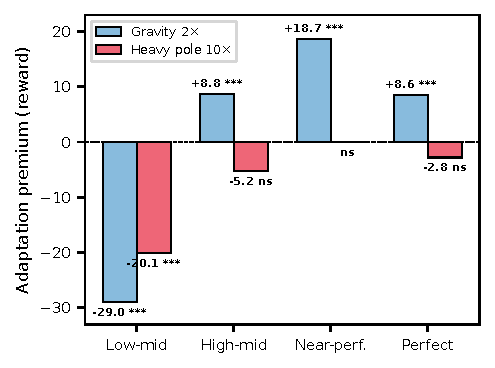
\includegraphics[width=\columnwidth]{figures/adaptation_premium_cross_variant.pdf}
  \caption{CartPole adaptation premium (non-stationary plasticity benefit minus static plasticity benefit) for two perturbation types. Gravity-2$\times$ yields significant positive premiums for competent strata (***$p<0.001$), indicating genuine adaptation beyond static fine-tuning. Heavy-pole shows near-zero premiums (n.s.).}
  \label{fig:adaptation}
\end{figure}

Under both variants, 88--90\% of High-mid networks benefit from plasticity in Phase~2 (post-perturbation). The gravity-2$\times$ variant yields a significant \emph{adaptation premium} (non-stationary benefit minus static benefit): $+8.8$ to $+18.7$ mean reward for competent strata ($p < 0.001$, Wilcoxon; Figure~\ref{fig:adaptation}), while heavy-pole shows near-zero premiums. Weight-change dynamics differ accordingly: under gravity-2$\times$, mean $|\Delta w|$ increases post-switch (ratio 1.13), consistent with active adaptation; under heavy-pole, it decreases (ratio 0.82--0.93), suggesting robustness rather than new adaptation.

\textbf{Causal confirmation via OFF$\to$ON.} To isolate adaptation from robustness, we disabled plasticity during Phase~1 and enabled it only at the switch point. OFF$\to$ON retains 66--69\% of the always-on benefit: 84--86\% of High-mid networks still improve, with oracle gains of $+53.9$ (heavy-pole) and $+59.9$ (gravity-2$\times$), representing \emph{pure} within-lifetime adaptation. A dose-response experiment varying switch time (100--400 steps) under heavy-pole confirms: benefit scales monotonically with post-switch duration (Spearman $\rho = 1.0$, all strata), from $+6.1$ at 100~steps to $+74.2$ at 400.

\subsection{Replication on Acrobot}
\label{sec:acrobot}

To test whether these findings generalise beyond CartPole, we repeated the analysis on Acrobot-v1, a harder control task with 6-dimensional observations and 3 discrete actions. We sampled 5{,}000 random genomes on a $20 \times 20$ developmental grid; 89.7\% were non-functional, leaving 513 networks across four performance strata, of which 87 (1.7\%) meet Gymnasium's solved threshold. Under per-network oracle tuning across a combined parameter grid (coarse 22-point + extended micro-$\eta$ dense sweep), 93--97\% of networks per stratum improve with plasticity (Table~\ref{tab:acrobot}). Acrobot requires substantially smaller learning rates than CartPole: the optimal $|\eta|$ is $10^{-4}$--$10^{-3}$ with high decay ($\lambda = 0.05$--$0.1$), roughly 10--100$\times$ smaller than CartPole's sweet spot. Yet regret under any fixed parameter is 100\%: no single $(\eta, \lambda)$ improves the average network, even on the extended grid. Plasticity is beneficial but entirely topology-dependent.

The anti-Hebbian picture is more nuanced on Acrobot (Table~\ref{tab:acrobot}). Cohen's $d$ favours anti-Hebbian across all strata ($d = 0.09$--$0.48$), but the per-network optimal $\eta$ splits roughly evenly between signs (151 anti-Hebbian vs 185 Hebbian). Under non-stationarity (2$\times$ lower-link mass at step~50) with the combined grid, 87--96\% of networks per stratum benefit from per-network oracle plasticity---again with 100\% regret under any fixed setting. Plasticity accelerates solving across all strata (Figure~\ref{fig:acrobot_survival}): the fraction of unsolved episodes at step~300 drops from 66\% to 40\% (High-mid) and from 31\% to 18\% (Near-perfect) compared to the no-plasticity baseline. These results show that the development-plasticity interaction is not benchmark-specific: topology-dependent plasticity holds on a task with richer dynamics, though the non-stationary benefit requires per-network tuning on the current grid.

\begin{table}[t]
\caption{Acrobot-v1 plasticity characterisation. \% Impr.: per-network oracle improvement rate on the combined grid (coarse + micro-$\eta$). Cohen's $d$: anti-Hebbian vs Hebbian (coarse grid). NS: non-stationary oracle rate (combined grid). Regret is 100\% under any fixed $(\eta, \lambda)$.}
\label{tab:acrobot}
\small
\begin{tabular}{@{}lrrrr@{}}
\toprule
Stratum & $N$ & \% Impr. & Cohen's $d$ & NS \% Helped \\
\midrule
Low-mid       & 71  & 95.8\% & $+0.48$*** & 88.7\% \\
High-mid      & 74  & 93.2\% & $+0.31$*** & 95.9\% \\
Near-perf.    & 281 & 93.6\% & $+0.15$*** & 86.8\% \\
Perfect       & 87  & 96.6\% & $+0.09$*   & 95.4\% \\
\bottomrule
\multicolumn{5}{@{}l@{}}{\footnotesize ***$p<0.001$, *$p<0.05$}
\end{tabular}
\end{table}

\begin{figure}[t]
  \centering
  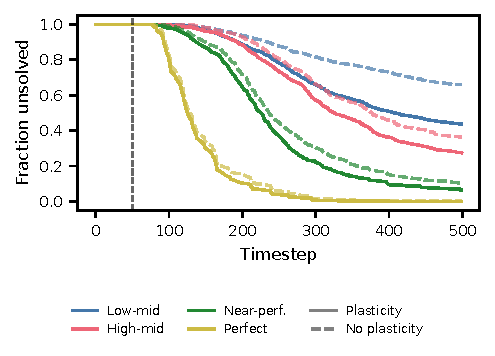
\includegraphics[width=\columnwidth]{figures/acrobot_survival.pdf}
  \caption{Acrobot fraction of episodes unsolved over time under non-stationarity (2$\times$ link mass at step~50). Solid: per-network oracle plasticity; dashed: no plasticity. Lower is better. Oracle plasticity accelerates solving across all strata---most visibly for High-mid and Near-perfect, where the unsolved fraction at step~300 drops from 66\%/31\% (no plasticity) to 40\%/18\% (oracle plasticity).}
  \label{fig:acrobot_survival}
\end{figure}

%% ============================================================
\section{Evolutionary Validation and Controls}
\label{sec:evolution}

\subsection{Co-Evolution Recovers Characterisation Findings}
\label{sec:coevol_results}

On CartPole, all three conditions converge to perfect fitness (reward~500) within 1--2 generations---the benchmark is too easy to differentiate conditions on final fitness ($p = 1.0$, Mann-Whitney). However, the evolved plasticity parameters reveal a clear signal. Starting from a uniform prior over $[-0.5, +0.5]$, \textbf{21/30 (70\%) of Condition~C runs evolve negative $\eta$} (binomial sign test $p = 0.043$), with median evolved $\eta = -0.117$ and population-mean $\eta$ drifting below zero within $\sim$10 generations (Figure~\ref{fig:eta_evolution}). Evolution independently discovers anti-Hebbian dominance. Co-evolution also produces sparser networks than no-plasticity evolution (median 277 vs 328 connections, $p = 0.10$, Mann-Whitney; neuron count identical at 100). The trend is stronger against fixed-plasticity evolution (277 vs 357, $p = 0.004$), hinting at a Baldwin-like effect where lifetime plasticity relaxes structural requirements.

On static Acrobot, no condition breaks through the architectural ceiling: all plateau at fitness~$\approx 0.84$ (reward~$\approx -78$), with all 90 runs in the High-mid stratum ($p \ge 0.72$, all pairwise comparisons). The critical finding is in the evolved $\eta$ distribution, which is \textbf{qualitatively different from CartPole}: median $\eta = -0.0045$, mean $\approx 0$, with 18/30 (60\%) negative ($p = 0.36$, n.s.). Evolved $|\eta|$ clusters in $[10^{-3}, 5 \times 10^{-2}]$---the Acrobot sweet spot from the characterisation (Section~\ref{sec:acrobot}). The cross-task contrast is itself informative: evolution finds different answers for different tasks, exactly as the characterisation predicts.

Under non-stationarity (2$\times$ lower-link mass at step~50), co-evolu\-tion is \textbf{counterproductive}: Condition~C (median fitness 0.775) is marginally worse than Condition~A (0.786; $d = 0.60$, $p = 0.033$ uncorrected, $p = 0.10$ after Bonferroni) and converges $3\times$ slower (median generation 10 vs 3 to reach fitness~0.75). The larger search space (56 vs 54 parameters) slows exploration without compensating fitness gains. The GA finds topologies that handle the perturbation through structure alone---Condition~A matches Condition~B---confirming that evolutionary architecture search absorbs non-stationarity without needing plasticity.

\begin{figure}[t]
  \centering
  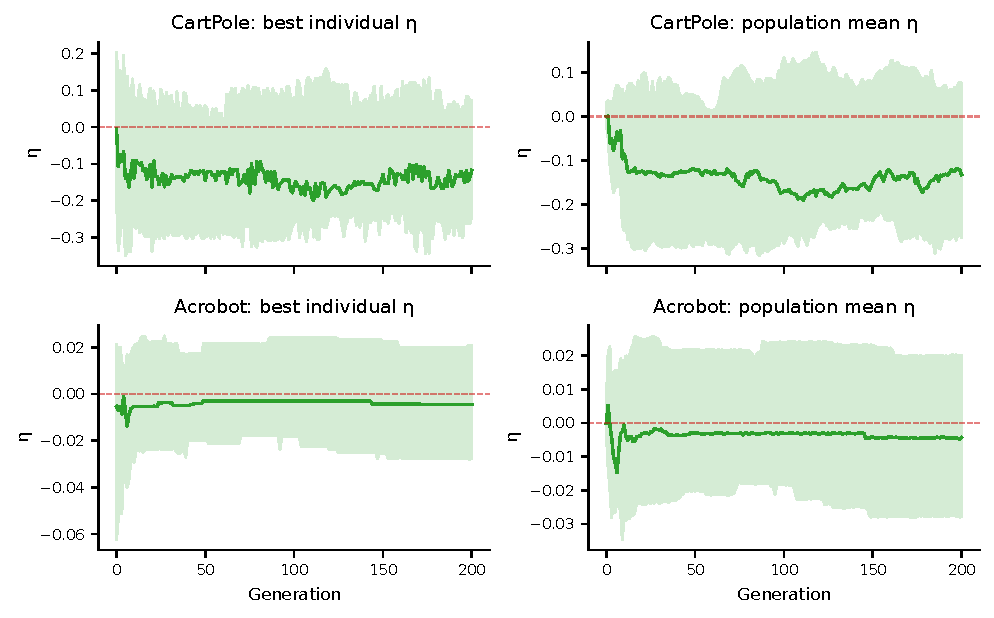
\includegraphics[width=\columnwidth]{figures/eta_evolution.pdf}
  \caption{Co-evolution (Condition~C) evolved $\eta$ over 200 generations on CartPole (top) and Acrobot (bottom). Left: best individual's $\eta$; right: population mean $\eta$ (median $\pm$ IQR across 30 runs). CartPole: strong anti-Hebbian drift ($\eta < 0$). Acrobot: $\eta$ hovers near zero with mixed signs, matching the characterisation finding.}
  \label{fig:eta_evolution}
\end{figure}

\subsection{Random-RNN Control}
\label{sec:random_results}

The random-RNN control (Section~\ref{sec:random_rnn_design}) yields three results that disambiguate developmental from generic network effects.

\textbf{Developmental competence advantage.} Of 11{,}810 random RNNs matched to competent MorphoNAS topologies, only 65 (0.56\%) are themselves competent (Low-mid: 17, High-mid: 18, Near-perfect: 4, Perfect: 26), compared to MorphoNAS's 4.7\%---an $8.4\times$ difference. Morphogenetic development provides a genuine structural inductive bias beyond topology statistics alone.

\textbf{Anti-Hebbian dominance is generic.} Anti-Hebbian plasticity dominates for competent random RNNs \emph{even more strongly} than for MorphoNAS networks: Cohen's $d = 1.67$ [95\% bootstrap CI: 1.57, 1.78] for High-mid and $d = 1.79$ [1.69, 1.90] for Low-mid, vs $d = 0.64$ and $d = 0.53$ for MorphoNAS. The magnitude-moderation mechanism operates regardless of how the network was wired; anti-Hebbian dominance is a property of small recurrent networks on CartPole, not of developmental topology specifically.

\textbf{Topology-dependence \emph{is} developmental-specific.} Regret under fixed parameters is substantially higher for MorphoNAS networks: 86\% (High-mid) vs 40\% for random RNNs, and 89\% (Near-perfect) vs 14\%. Morphogenetic development creates more diverse topology-plasticity interactions, making per-network tuning---or co-evolution---more important for developmental systems than for random architectures.

%% ============================================================
\section{Discussion and Conclusion}
\label{sec:discussion}

The combination of characterisation, co-evolutionary validation, and random-RNN control allows us to separate general from deve\-lopmental-specific findings with unusual precision.

\textbf{Separating general from developmental-specific findings.} The random-RNN control (Section~\ref{sec:random_results}) resolves a question that the characterisation alone could not answer. Anti-Hebbian dominance turns out to be a generic property of small recurrent networks---the magnitude-moderation mechanism operates regardless of wiring origin. This recontextualises the characterisation finding: practitioners should default to anti-Hebbian plasticity not because of anything specific to developmental topology, but because it prevents runaway weight growth in any small RNN. By contrast, the \emph{degree} of topology-dependence is genuinely developmental: the $2$--$6\times$ higher regret for MorphoNAS networks means that morphogenetic development creates a uniquely diverse phenotype space where per-network tuning (or co-evolution) is far more important than for random architectures.

\textbf{Co-evolution recovers characterisation patterns but does not improve fitness.} On no benchmark or condition does co-evolution improve fitness over no-plasticity evolution (Section~\ref{sec:coevol_results}). Under non-stationarity, co-evolution is marginally \emph{worse} ($d = 0.60$): the two extra parameters slow convergence without payoff, because the GA finds topologies robust to the perturbation through structure alone. This reinforces a central finding: \emph{topology is the primary determinant of performance}---plasticity improves a given topology (characterisation) but does not help the evolutionary search for topology. The scientific contribution is methodological: evolution independently recovers the characterisation findings (anti-Hebbian on CartPole, mixed-sign near-zero on Acrobot, correct $\eta$ scale) without prior knowledge. The $8.4\times$ developmental competence advantage (Section~\ref{sec:random_results}) further underscores that reaction-diffusion development provides structural inductive bias beyond topology statistics alone.

\textbf{Implications for evolving self-organisation.} Our findings connect structural self-organisation (development) with functional self-organisation (plasticity) through evolution. In NDP~\cite{najarro2023ndp} and HyperNCA~\cite{najarro2022hypernca}, development is driven by learned update rules; Plantec et~al.~\cite{plantec2024evolving} showed that structural plasticity can extend development into the lifetime. Our results demonstrate that even simple synaptic plasticity provides substantial benefits on top of morphogenetic development, and that evolutionary optimisation can discover the appropriate plasticity parameters for each task. The sparser architectures evolved under co-evolution on CartPole (277 vs 357 connections compared to fixed-plasticity evolution, $p = 0.004$; Section~\ref{sec:coevol_results}) suggest a Baldwin-like effect where lifetime plasticity relaxes the structural requirements on the genome---a direction worth pursuing on harder benchmarks.

\textbf{Practical guidelines.} (1)~Default to anti-Hebbian plasticity ($\eta < 0$) with moderate decay ($\lambda \approx 0.01$)---this is both the characterisation recommendation and what evolution discovers independently. (2)~Invest in per-network parameter tuning: regret under fixed parameters is 52--100\% for MorphoNAS networks, far higher than for random architectures. (3)~When targeting non-stationary environments, the OFF$\to$ON protocol shows that adaptation alone accounts for 66--69\% of the total benefit.

\textbf{Limitations.} Both benchmarks are classic control tasks; generalisation to continuous-action or high-dimensional environments remains open. Co-evolution never outperforms no-plasticity evolution, and is marginally counterproductive under non-stationarity---a stronger test would use a benchmark where the GA cannot find robust topologies within 200 generations, forcing reliance on within-lifetime adaptation. The random-RNN sample is small (65 competent networks), and the weight distribution differs from MorphoNAS (uniform vs distance-dependent), introducing a potential confound. The plasticity rule (Eq.~\ref{eq:hebb}) is deliberately simple; richer mechanisms~\cite{soltoggio2018born} may interact differently with developmental topologies.

\textbf{Broader context.} Zador~\cite{zador2019critique} argued that biological brains leverage both genomic encoding and environmental interaction. Shuvaev et~al.~\cite{shuvaev2024encoding} confirmed this computationally, showing that small genomic networks can compress weight matrices by orders of magnitude while retaining substantial task performance. Our findings extend this picture with empirical evidence: the morphogenetic genome provides the compressed architectural scaffold (with an $8.4\times$ competence advantage over random wiring), plasticity provides within-lifetime adaptation, and evolution can discover appropriate plasticity parameters for each task. Across all experiments, the primary determinant of performance remains the developmental topology itself.

\begin{acks}
AI-assisted tools (Claude, Anthropic) were used to write and debug experimental and analysis code under author direction, and to edit and polish the manuscript text. All scientific decisions---including experimental design, data interpretation, and conclusions---are the authors' own. Source code and data are available at \url{https://github.com/ukma-morphonas-lab/MorphoNAS-PL}.
\end{acks}

%%% Bibliography inlined from main.bbl for arXiv compatibility
\begin{thebibliography}{18}

\ifx \showCODEN    \undefined \def \showCODEN     #1{\unskip}     \fi
\ifx \showISBNx    \undefined \def \showISBNx     #1{\unskip}     \fi
\ifx \showISBNxiii \undefined \def \showISBNxiii  #1{\unskip}     \fi
\ifx \showISSN     \undefined \def \showISSN      #1{\unskip}     \fi
\ifx \showLCCN     \undefined \def \showLCCN      #1{\unskip}     \fi
\ifx \shownote     \undefined \def \shownote      #1{#1}          \fi
\ifx \showarticletitle \undefined \def \showarticletitle #1{#1}   \fi
\ifx \showURL      \undefined \def \showURL       {\relax}        \fi
\providecommand\bibfield[2]{#2}
\providecommand\bibinfo[2]{#2}
\providecommand\natexlab[1]{#1}
\providecommand\showeprint[2][]{arXiv:#2}

\bibitem[Derrac et~al\mbox{.}(2011)]%
        {derrac2011practical}
\bibfield{author}{\bibinfo{person}{Joaqu{\'\i}n Derrac},
  \bibinfo{person}{Salvador Garc{\'\i}a}, \bibinfo{person}{Daniel Molina},
  {and} \bibinfo{person}{Francisco Herrera}.} \bibinfo{year}{2011}\natexlab{}.
\newblock \showarticletitle{A practical tutorial on the use of nonparametric
  statistical tests as a methodology for comparing evolutionary and swarm
  intelligence algorithms}.
\newblock \bibinfo{journal}{\emph{Swarm and Evolutionary Computation}}
  \bibinfo{volume}{1}, \bibinfo{number}{1} (\bibinfo{year}{2011}),
  \bibinfo{pages}{3--18}.
\newblock
\href{https://doi.org/10.1016/j.swevo.2011.02.002}{doi:\nolinkurl{10.1016/j.swevo.2011.02.002}}


\bibitem[Garc{\'\i}a~N{\'u}{\~n}ez et~al\mbox{.}(2025)]%
        {garcianunez2025time}
\bibfield{author}{\bibinfo{person}{Daniel Garc{\'\i}a~N{\'u}{\~n}ez},
  \bibinfo{person}{Fergal Stapleton}, {and} \bibinfo{person}{Edgar
  Galv{\'a}n}.} \bibinfo{year}{2025}\natexlab{}.
\newblock \showarticletitle{Time-Modulated {H}ebbian Learning for Classic
  Control Tasks}. In \bibinfo{booktitle}{\emph{GECCO '25 Companion: Proceedings
  of the Genetic and Evolutionary Computation Conference Companion}}.
  \bibinfo{publisher}{ACM}, \bibinfo{pages}{2119--2126}.
\newblock
\href{https://doi.org/10.1145/3712255.3734322}{doi:\nolinkurl{10.1145/3712255.3734322}}


\bibitem[Glybovets and Medvid(2026)]%
        {glybovets2026morphonas}
\bibfield{author}{\bibinfo{person}{Mykola Glybovets} {and}
  \bibinfo{person}{Sergii Medvid}.} \bibinfo{year}{2026}\natexlab{}.
\newblock \showarticletitle{{MorphoNAS}: Embryogenic Neural Architecture Search
  Through Morphogen-Guided Development}.
\newblock \bibinfo{journal}{\emph{Kibernetyka i Systemnyj Analiz (Cybernetics
  and Systems Analysis)}} \bibinfo{volume}{62}, \bibinfo{number}{2}
  (\bibinfo{year}{2026}).
\newblock
\href{https://doi.org/10.34229/KCA2522-9664.26.2.3}{doi:\nolinkurl{10.34229/KCA2522-9664.26.2.3}}
\newblock
\shownote{Preprint: arXiv:2507.13785}.


\bibitem[Hebb(1949)]%
        {hebb1949organization}
\bibfield{author}{\bibinfo{person}{Donald~O Hebb}.}
  \bibinfo{year}{1949}\natexlab{}.
\newblock \bibinfo{booktitle}{\emph{The Organization of Behavior: A
  Neuropsychological Theory}}.
\newblock \bibinfo{publisher}{Wiley}.
\newblock


\bibitem[Mordvintsev et~al\mbox{.}(2020)]%
        {mordvintsev2020growing}
\bibfield{author}{\bibinfo{person}{Alexander Mordvintsev},
  \bibinfo{person}{Ettore Randazzo}, \bibinfo{person}{Eyvind Niklasson}, {and}
  \bibinfo{person}{Michael Levin}.} \bibinfo{year}{2020}\natexlab{}.
\newblock \showarticletitle{Growing Neural Cellular Automata}.
\newblock \bibinfo{journal}{\emph{Distill}} \bibinfo{volume}{5},
  \bibinfo{number}{2} (\bibinfo{year}{2020}), \bibinfo{pages}{e23}.
\newblock
\href{https://doi.org/10.23915/distill.00023}{doi:\nolinkurl{10.23915/distill.00023}}


\bibitem[Najarro and Risi(2020)]%
        {najarro2020meta}
\bibfield{author}{\bibinfo{person}{Elias Najarro} {and}
  \bibinfo{person}{Sebastian Risi}.} \bibinfo{year}{2020}\natexlab{}.
\newblock \showarticletitle{Meta-Learning through Hebbian Plasticity in Random
  Networks}. In \bibinfo{booktitle}{\emph{Advances in Neural Information
  Processing Systems}}, Vol.~\bibinfo{volume}{33}.
  \bibinfo{pages}{20719--20731}.
\newblock


\bibitem[Najarro et~al\mbox{.}(2022)]%
        {najarro2022hypernca}
\bibfield{author}{\bibinfo{person}{Elias Najarro}, \bibinfo{person}{Shyam
  Sudhakaran}, \bibinfo{person}{Claire Glanois}, {and}
  \bibinfo{person}{Sebastian Risi}.} \bibinfo{year}{2022}\natexlab{}.
\newblock \showarticletitle{{HyperNCA}: Growing Developmental Networks with
  Neural Cellular Automata}. In \bibinfo{booktitle}{\emph{From Cells to
  Societies: Collective Learning Across Scales (ICLR 2022 Workshop)}}.
\newblock


\bibitem[Najarro et~al\mbox{.}(2023)]%
        {najarro2023ndp}
\bibfield{author}{\bibinfo{person}{Elias Najarro}, \bibinfo{person}{Shyam
  Sudhakaran}, {and} \bibinfo{person}{Sebastian Risi}.}
  \bibinfo{year}{2023}\natexlab{}.
\newblock \showarticletitle{Towards Self-Assembling Artificial Neural Networks
  through Neural Developmental Programs}. In
  \bibinfo{booktitle}{\emph{Proceedings of the 2023 Artificial Life Conference
  (ALIFE)}}, Vol.~\bibinfo{volume}{35}. \bibinfo{publisher}{MIT Press},
  \bibinfo{pages}{80}.
\newblock
\href{https://doi.org/10.1162/isal_a_00693}{doi:\nolinkurl{10.1162/isal_a_00693}}


\bibitem[Nisioti et~al\mbox{.}(2024)]%
        {nisioti2024growing}
\bibfield{author}{\bibinfo{person}{Eleni Nisioti}, \bibinfo{person}{Erwan
  Plantec}, \bibinfo{person}{Milton Montero}, \bibinfo{person}{Joachim~Winther
  Pedersen}, {and} \bibinfo{person}{Sebastian Risi}.}
  \bibinfo{year}{2024}\natexlab{}.
\newblock \showarticletitle{Growing Artificial Neural Networks for Control: the
  Role of Neuronal Diversity}. In \bibinfo{booktitle}{\emph{GECCO '24
  Companion: Proceedings of the Genetic and Evolutionary Computation Conference
  Companion}}. \bibinfo{publisher}{ACM}, \bibinfo{pages}{175--178}.
\newblock
\href{https://doi.org/10.1145/3638530.3654356}{doi:\nolinkurl{10.1145/3638530.3654356}}


\bibitem[Palm et~al\mbox{.}(2021)]%
        {palm2021testing}
\bibfield{author}{\bibinfo{person}{Rasmus~Berg Palm}, \bibinfo{person}{Elias
  Najarro}, {and} \bibinfo{person}{Sebastian Risi}.}
  \bibinfo{year}{2021}\natexlab{}.
\newblock \showarticletitle{Testing the Genomic Bottleneck Hypothesis in
  {H}ebbian Meta-Learning}. In \bibinfo{booktitle}{\emph{Proceedings of Machine
  Learning Research}}, Vol.~\bibinfo{volume}{148}. \bibinfo{pages}{100--110}.
\newblock


\bibitem[Plantec et~al\mbox{.}(2024)]%
        {plantec2024evolving}
\bibfield{author}{\bibinfo{person}{Erwan Plantec},
  \bibinfo{person}{Joachim~Winther Pedersen}, \bibinfo{person}{Milton~Llera
  Montero}, \bibinfo{person}{Eleni Nisioti}, {and} \bibinfo{person}{Sebastian
  Risi}.} \bibinfo{year}{2024}\natexlab{}.
\newblock \showarticletitle{Evolving Self-Assembling Neural Networks: From
  Spontaneous Activity to Experience-Dependent Learning}. In
  \bibinfo{booktitle}{\emph{Proceedings of the 2024 Conference on Artificial
  Life}}. \bibinfo{publisher}{MIT Press}.
\newblock


\bibitem[Shuvaev et~al\mbox{.}(2024)]%
        {shuvaev2024encoding}
\bibfield{author}{\bibinfo{person}{Sergey Shuvaev}, \bibinfo{person}{Divyansha
  Lachi}, \bibinfo{person}{Alexei Koulakov}, {and} \bibinfo{person}{Anthony
  Zador}.} \bibinfo{year}{2024}\natexlab{}.
\newblock \showarticletitle{Encoding innate ability through a genomic
  bottleneck}.
\newblock \bibinfo{journal}{\emph{Proceedings of the National Academy of
  Sciences}} \bibinfo{volume}{121}, \bibinfo{number}{38}
  (\bibinfo{year}{2024}), \bibinfo{pages}{e2409160121}.
\newblock
\href{https://doi.org/10.1073/pnas.2409160121}{doi:\nolinkurl{10.1073/pnas.2409160121}}


\bibitem[Soltoggio et~al\mbox{.}(2018)]%
        {soltoggio2018born}
\bibfield{author}{\bibinfo{person}{Andrea Soltoggio},
  \bibinfo{person}{Kenneth~O Stanley}, {and} \bibinfo{person}{Sebastian Risi}.}
  \bibinfo{year}{2018}\natexlab{}.
\newblock \showarticletitle{Born to learn: the inspiration, progress, and
  future of evolved plastic artificial neural networks}.
\newblock \bibinfo{journal}{\emph{Neural Networks}}  \bibinfo{volume}{108}
  (\bibinfo{year}{2018}), \bibinfo{pages}{48--67}.
\newblock
\href{https://doi.org/10.1016/j.neunet.2018.07.013}{doi:\nolinkurl{10.1016/j.neunet.2018.07.013}}


\bibitem[Stanley et~al\mbox{.}(2009)]%
        {stanley2009hypercube}
\bibfield{author}{\bibinfo{person}{Kenneth~O Stanley}, \bibinfo{person}{David~B
  D'Ambrosio}, {and} \bibinfo{person}{Jason Gauci}.}
  \bibinfo{year}{2009}\natexlab{}.
\newblock \showarticletitle{A Hypercube-Based Encoding for Evolving Large-Scale
  Neural Networks}.
\newblock \bibinfo{journal}{\emph{Artificial Life}} \bibinfo{volume}{15},
  \bibinfo{number}{2} (\bibinfo{year}{2009}), \bibinfo{pages}{185--212}.
\newblock


\bibitem[Stanley and Miikkulainen(2002)]%
        {stanley2002evolving}
\bibfield{author}{\bibinfo{person}{Kenneth~O Stanley} {and}
  \bibinfo{person}{Risto Miikkulainen}.} \bibinfo{year}{2002}\natexlab{}.
\newblock \showarticletitle{Evolving Neural Networks through Augmenting
  Topologies}.
\newblock \bibinfo{journal}{\emph{Evolutionary Computation}}
  \bibinfo{volume}{10}, \bibinfo{number}{2} (\bibinfo{year}{2002}),
  \bibinfo{pages}{99--127}.
\newblock


\bibitem[Towers et~al\mbox{.}(2024)]%
        {towers2024gymnasium}
\bibfield{author}{\bibinfo{person}{Mark Towers}, \bibinfo{person}{Ariel
  Kwiatkowski}, \bibinfo{person}{Jordan Terry}, \bibinfo{person}{John~U Balis},
  \bibinfo{person}{Gianluca De~Cola}, \bibinfo{person}{Tristan Deleu},
  \bibinfo{person}{Manuel Goul{\~a}o}, \bibinfo{person}{Andreas Kallinteris},
  \bibinfo{person}{Arjun KG}, \bibinfo{person}{Markus Krimmel},
  \bibinfo{person}{Rodrigo Perez-Vicente}, \bibinfo{person}{Andrea Pierr{\'e}},
  \bibinfo{person}{Sander Schulhoff}, \bibinfo{person}{Jun~Jet Tai},
  \bibinfo{person}{Andrew Tan}, {and} \bibinfo{person}{Omar~G Younis}.}
  \bibinfo{year}{2024}\natexlab{}.
\newblock \bibinfo{booktitle}{\emph{Gymnasium}}.
\newblock
\urldef\tempurl%
\url{https://github.com/Farama-Foundation/Gymnasium}
\showURL{%
\tempurl}


\bibitem[Turing(1952)]%
        {turing1952chemical}
\bibfield{author}{\bibinfo{person}{Alan~M Turing}.}
  \bibinfo{year}{1952}\natexlab{}.
\newblock \showarticletitle{The Chemical Basis of Morphogenesis}.
\newblock \bibinfo{journal}{\emph{Philosophical Transactions of the Royal
  Society of London. Series B, Biological Sciences}} \bibinfo{volume}{237},
  \bibinfo{number}{641} (\bibinfo{year}{1952}), \bibinfo{pages}{37--72}.
\newblock
\href{https://doi.org/10.1098/rstb.1952.0012}{doi:\nolinkurl{10.1098/rstb.1952.0012}}


\bibitem[Zador(2019)]%
        {zador2019critique}
\bibfield{author}{\bibinfo{person}{Anthony~M Zador}.}
  \bibinfo{year}{2019}\natexlab{}.
\newblock \showarticletitle{A critique of pure learning and what artificial
  neural networks can learn from animal brains}.
\newblock \bibinfo{journal}{\emph{Nature Communications}} \bibinfo{volume}{10},
  \bibinfo{number}{1} (\bibinfo{year}{2019}), \bibinfo{pages}{3770}.
\newblock
\href{https://doi.org/10.1038/s41467-019-11786-6}{doi:\nolinkurl{10.1038/s41467-019-11786-6}}


\end{thebibliography}

\end{document}
